\documentclass[review,preprint]{elsarticle}

%% Use the option review to obtain double line spacing
%% \documentclass[authoryear,preprint,review,12pt]{elsarticle}

%% Use the options 1p,twocolumn; 3p; 3p,twocolumn; 5p; or 5p,twocolumn
%% for a journal layout:
%% \documentclass[final,1p,times]{elsarticle}
%% \documentclass[final,1p,times,twocolumn]{elsarticle}
%% \documentclass[final,3p,times]{elsarticle}
%% \documentclass[final,3p,times,twocolumn]{elsarticle}
%% \documentclass[final,5p,times]{elsarticle}
%% \documentclass[final,5p,times,twocolumn]{elsarticle}


\usepackage[final]{changes}

\usepackage{hyperref}
\usepackage{amsmath}
\usepackage{amssymb}
\usepackage{braket}
\usepackage{siunitx}
\usepackage[version=4]{mhchem}
\usepackage{tikz}
\usetikzlibrary{positioning}
\usetikzlibrary {arrows.meta} 
\usepackage{paralist}
\usepackage{todonotes}
\usepackage{tabularray}

\DeclareMathOperator{\erf}{erf}

%% The lineno packages adds line numbers. Start line numbering with
%% \begin{linenumbers}, end it with \end{linenumbers}. Or switch it on
%% for the whole article with \linenumbers.
%\usepackage{lineno}
%\linenumbers

\journal{Chemical Physics Impact}

\begin{document}
	
	\begin{frontmatter}
		
		%% Title, authors and addresses
		
		\title{Reaction at calcium anode}
		
		\author[1]{Pierre Beaujean\corref{cor1}}
		
		\ead{pierre.beaujean@unamur.be}
		
		\cortext[cor1]{Corresponding author}
		
		\affiliation[1]{organization={Theoretical Chemistry Laboratory, Unit of Theoretical and Structural Physical Chemistry, Namur Institute of Structured Matter, University of Namur},%Department and Organization
			addressline={Rue de Bruxelles, 61}, 
			city={Namur},
			postcode={B-5000}, 
			country={Belgium}}
			
			\author[1]{Benoît Champagne}
		
		\begin{abstract}
			Probably.
		\end{abstract}
		
		
		%%Graphical abstract
%		\begin{graphicalabstract}
%			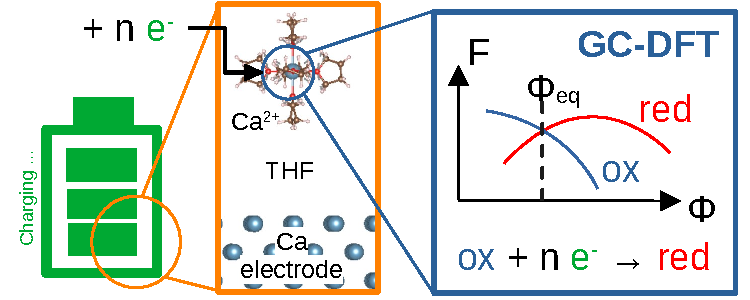
\includegraphics{Graphical_Abstract}
%		\end{graphicalabstract}
		
		%%Research highlights
%\begin{highlights}
%	\item  \replaced{Electrostatics of the substituents drives the nitroxide redox behavior}{Electrostatic interactions between the redox center and substituents strongly affect nitroxide redox potentials.}
%	\item \replaced{The nitroxide skeleton has a moderate influence (0.1 V) on the redox behavior}{The nitroxide skeleton has a moderate influence.}
%	\item \replaced{Electrolytes stabilize charged nitroxides and shift their redox potentials}{Electrolytes stabilize charged nitroxide species, leading to shifts in their redox potentials.}
%	\item \replaced{Ion-substituent (especially when aromatic) interactions enhance ion-pair stability}{Ion-substituent interactions, especially in aromatic systems, play a key role in ion-pair stability.}
%\end{highlights}
%
%		
%		\begin{keyword}
%			%% keywords here, in the form: keyword \sep keyword
%			Nitroxide 
%			\sep Electrolyte 
%			\sep Redox potential
%			\sep Debye-Hückel 
%			\sep Ion pairs 
%			\sep Quantum chemistry
%			
%			%% PACS codes here, in the form: \PACS code \sep code
%			
%			%% MSC codes here, in the form: \MSC code \sep code
%			%% or \MSC[2008] code \sep code (2000 is the default)
%			
%		\end{keyword}
		
	\end{frontmatter}
	
	% \linenumbers
	
%% main text

\section{Introduction}

\begin{itemize}
	\item it is important to understand SEI and computational chemistry can help here,
	\item M. L. Doublet et J. S. Filhol have developed a nice methodology and they have already tried in glyme \cite{nguyenSolvationReductionCoupling2023}
	\item We want to try in THF (to follow our previous publication) and with \ce{CaH2}.
\end{itemize}

\section{Computational details}

All calculations, including geometry optimizations and binding energy evaluations, are carried out using the Vienna \textit{Ab initio} Simulation Package (VASP, version 6.3.2), within the framework of density functional theory (DFT). The Perdew--Burke--Ernzerhof (PBE) exchange-correlation functional is employed in conjunction with the D3 dispersion correction and the projector augmented-wave (PAW) method~\cite{blochlProjectorAugmentedwaveMethod1994}. The \texttt{Ca\_pv} pseudopotential is used to model calcium~\cite{blochlProjectorAugmentedwaveMethod1994,kresseUltrasoftPseudopotentialsProjector1999}.
A kinetic energy cutoff of \SI{550}{\electronvolt} is applied to the plane-wave basis set. Brillouin zone integrations are performed using a $4 \times 4 \times 1$ Monkhorst-Pack $k$-point mesh~\cite{monkhorstSpecialPointsBrillouinzone1976}. Solvation effects from outer solvent molecules are included via the VASPSOL implicit solvation model~\cite{mathewImplicitSolvationModel2014,mathewImplicitSelfconsistentElectrolyte2019}, with the dielectric constant set to $\varepsilon_r = 7.56$ to represent tetrahydrofuran (THF). Following Filhol and co-workers~\cite{kopaclautarElectrolyteReactivityDouble2020,kopaclautarModelingInterfacialElectrochemistry2020,hagopianInitioModellingInterfacial2021,nguyenSolvationReductionCoupling2023}, the surface tension parameter is set to $\tau = 0$, the cavity is defined using a density cutoff of $\rho_K = 5 \times 10^{-5}$~\si{\per\angstrom\cubed}, and the cavity smearing parameter is kept at its default value of $\sigma_k = 0.6$.

All structural optimizations employ the Limited-memory Broyden-Flet\-cher\-Gol\-dfarb-Shanno (L-BFGS) algorithm, as implemented in the Atomic Simulation Environment (ASE) package~\cite{larsenAtomicSimulationEnvironment2017}. Forces and energies are obtained from VASP, and the optimizations proceed until all atomic forces fall below \SI{e-2}{\electronvolt\per\angstrom}. For solvated calcium species (i.e., the calcium atom and its first explicit solvation shell), the system is placed in a cubic box of \SI{20}{\angstrom} side length, centered on the molecular center of mass, with fixed cell dimensions during optimization.
Slab models are constructed from optimized bulk structures of \ce{Ca^0} (Materials Project ID: \texttt{MP-45}) and \ce{CaH2} (\texttt{MP-23713}), both relaxed with respect to atomic positions and cell parameters. From these, $3 \times 3$ and $2 \times 2$ slabs of the (100) surface of \ce{Ca^0} and \ce{CaH2}, respectively, are created. Each slab consists of six atomic layers and is separated from its periodic image by a vacuum region of \SI{52}{\angstrom} (to have room for the solvated structures, \textit{vide infra}). The slab terminations are selected to ensure non-polar surfaces, generated using ASE. They are then relaxed with frozen cell parameters.

Electrochemical interface effects are modeled in the grand canonical ensemble, using the formalism developed by Filhol \textit{et al.}~\cite{hagopianAdvancementHomogeneousBackground2022}, using a set of scripts available at \url{https://github.com/pierre-24/ec-interface/}. In each case, a symmetric unit cell is constructed by placing the optimized solvated structure on both sides of the slab, within the interfacial double-layer region, such that the atom closest to the surface is at a distance of \SI{9}{\angstrom} from it.
The electrochemical free energy $F(\Phi)$ is evaluated as a function of the electrochemical potential $\Phi$ through surface (dis)charging:
\begin{equation}
	F(\Phi) = H(\Phi) - q\Phi \approx E(\Delta n_e) - \Delta n_e \Phi(\Delta n_e),
\end{equation}
where $\Delta n_e$ denotes the change in electron number relative to the neutral system (in most of the cases, $-6 \leq \Delta n_e \leq 2$), $E(\Delta n_e)$ is the total energy under charge perturbation, and $\Phi(\Delta n_e)$ is the corresponding work function. The latter is computed as
\begin{equation*}
	\Phi(\Delta n_e) = E_\infty(\Delta n_e) - E_F(\Delta n_e),
\end{equation*}
with $E_\infty$ and $E_F$ denoting the vacuum and Fermi levels, respectively. These absolute potentials are converted to the standard hydrogen electrode (SHE) by using $E^0_{rel} = \Phi(\Delta n_e) - \SI{4.5}{\volt}$. Note that these charged systems are treated using the homogeneous background method (HBM)~\cite{hagopianAdvancementHomogeneousBackground2022} to account for the homogeneous background of charge added by VASP to maintain the neutrality of the unit cell. In this study, the fraction of active electrons set to $\alpha_s = 0.8$.  


\section{Results and discussion}

\begin{figure}[!h]
	\centering
	\includegraphics[width=.8\linewidth]{Figure1}
	\caption{Electrochemical curve.}
\end{figure}

\begin{itemize}
	\item Stripping/platting reaction curve in THF + number of electron exchanged + fukui analysis.
	\item Possible side product, based on the previous analysis: reaction energies, a bit of geometrical analysis.
	\item Further curves (probably only the main byproduct, using PZC for the others?) + \ce{CaH2}.
\end{itemize}

\begin{figure}[!h]
\centering
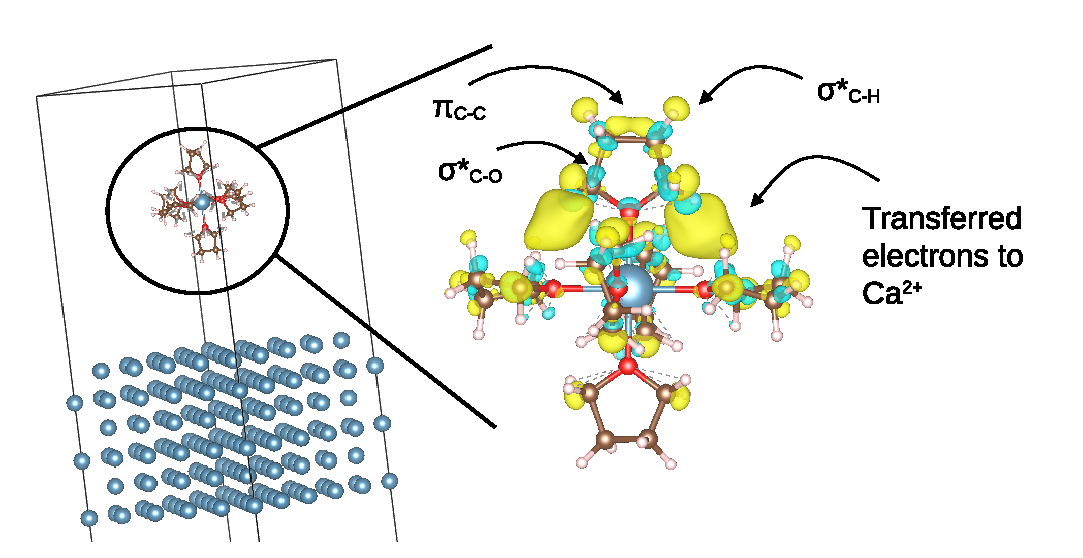
\includegraphics[width=.8\linewidth]{Figure2}
\caption{Fukui function}
\end{figure}

\section{Conclusions}

X.

\clearpage
\section*{CRediT authorship contribution statement}

\textbf{Pierre Beaujean:} Conceptualization, Methodology, Software, Validation, Formal analysis, Investigation, Data Curation, Writing - Original Draft, Writing - Review \& Editing, Visualization.

\textbf{Benoît Champagne:} xxx.
	
\section*{Declaration of competing interest}

The author declares that he has no known competing financial interests or personal relationships that could have appeared to influence the work reported in this paper

\section*{Acknowledgements}
This work was supported by the Excellence of Science (EOS) programme  ECOBAT (EOS No. 40007515). 
The calculations were performed on: \begin{inparaenum}[(i)]
	\item the computers of the Consortium des \'{E}quipements de Calcul Intensif (C\'{E}CI, \url{http://www.ceci-hpc.be}) and particularly those of the Technological Platform of High-Performance Computing, for which the author gratefully acknowledge the financial support of the F.R.S-FNRS, of the Walloon Region, and of the University of Namur (Conventions No. 2.5020.11, U.G006.15, U.G018.19, U.G011.22, 1610468, and RW/GEQ2016), and
	\item on Lucia, the Tier-1 supercomputer of the Walloon Region, infrastructure funded by the Walloon Region (grant agreement No. 1910247).
\end{inparaenum} 

\section*{Data availability}

XXX.
	

\bibliographystyle{elsarticle-num-names} 
\bibliography{biblio}
	
\end{document}
\endinput
%%
%% End of file `elsarticle-template-num.tex'.
